\documentclass{article}
\usepackage[letterpaper,top=2cm,bottom=2cm,left=3cm,right=3cm,marginparwidth=1.75cm]{geometry}
\usepackage[russian]{babel}
\usepackage{amsmath}
\usepackage{graphicx}
\usepackage[utf8]{inputenc}
\usepackage[colorlinks=true, allcolors=blue]{hyperref}
\usepackage[pdf]{graphviz}
\graphicspath{ {./static/1/}{./static/2/}{./static/3/}}


\title{ТМВ Домашнее задание №1}
\author{А-13б-19 Головин Антон}
\date{7 апреля 2022}

\begin{document}
\maketitle
%%%%%%%%%%%%%%%%%%%%%%%%%%%%%% Задание 1 %%%%%%%%%%%%%%%%%%%%%%%%%%%%%%
\section{Задание №1. Построить конечный автомат, распознающий язык.}
\begin{enumerate}
%%%%%%%%%%%%%%% 1.1 %%%%%%%%%%%%%%%
\item {$L = \{ w \in \{a,b,c\}^*  $ | $  |w|_c = 1 \} $} \\
\begin{center}
    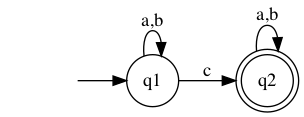
\includegraphics[width=0.5\textwidth]{g11.png}
\end{center}
%%%%%%%%%%%%%%% 1.2 %%%%%%%%%%%%%%%
\item {$L = \{ w \in \{a,b\}^*  $ | $  |w|_a \le 2, {|w|_b} \ge 2 \}$} \\ \\
Это задача на прямое произведение. \\ \\
$L_{11} = \{ w \in \{a,b\}^*  $ | $  |w|_a \le 2 \} $\\
\begin{center}
    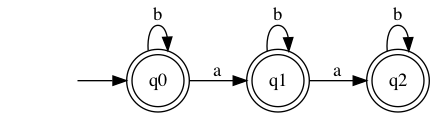
\includegraphics[width=0.5\textwidth]{g121.png}
\end{center}

$L_{12} = \{ w \in \{a,b\}^*  $ | $  |w|_b \ge 2 \} $
\begin{center}
    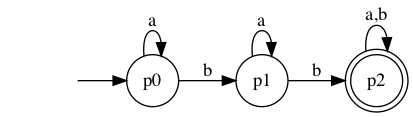
\includegraphics[width=0.5\textwidth]{g122.png}
\end{center}

\newpage

\begin{center}
\[
    L = L_{11} \times L_{12} \Rightarrow \]
    \[A_1 = \left\langle \sum_{1} , Q_1, S_1, T_1, \delta_1\right\rangle \quad 
    A_2 = \left\langle \sum_{2}, Q_2, S_2, T_2, \delta_2\right\rangle
\]

\[
    \sum = \{a, b\} \\
    Q = Q_1 \times Q_2 = \{q0p0, q0p1, q0p2, q1p0, q1p1, q1p2, q2p0, q2p1, q2p2\} \\
    S = \left\langle S_1, S_2\right\rangle = \left\langle q0,p0 \right\rangle \\
    T = T_1 \times T_2 = \left\langle q2p2, q1p2, q0p2 \right\rangle
\]

$$\delta(\left\langle q1,q2 \right\rangle, c) = \left\langle \delta_1(q_1, c), \delta_2(q_2, c)\right\rangle $$

\begin{tabular}{ |c|c|c| } 
    \hline
    & $a$ & $b$ \\
    \hline
    \left\langle q0,p0 \right\rangle & \left\langle q1,p0 \right\rangle & \left\langle q0,p1 \right\rangle \\
    \hline
    \left\langle q0,p1 \right\rangle & \left\langle q1,p1 \right\rangle & \left\langle q0,p2 \right\rangle \\
    \hline
    \left\langle q0,p2 \right\rangle & \left\langle q1,p2 \right\rangle & \left\langle q0,p2 \right\rangle \\
    \hline
    \left\langle q1,p0 \right\rangle & \left\langle q2,p0 \right\rangle & \left\langle q1,p0 \right\rangle \\
    \hline
    \left\langle q1,p1 \right\rangle & \left\langle q2,p1 \right\rangle & \left\langle q1,p2 \right\rangle \\
    \hline
    \left\langle q1,p2 \right\rangle & \left\langle q2,p2 \right\rangle & \left\langle q1,p2 \right\rangle \\
    \hline
    \left\langle q2,p0 \right\rangle &  -  & \left\langle q2,p1 \right\rangle \\
    \hline
    \left\langle q2,p1 \right\rangle &  -  & \left\langle q2,p2 \right\rangle \\
    \hline
    \left\langle q2,p2 \right\rangle &  -  & \left\langle q2,p2 \right\rangle \\
    \hline
\end{tabular}
\end{center}

\begin{center}
    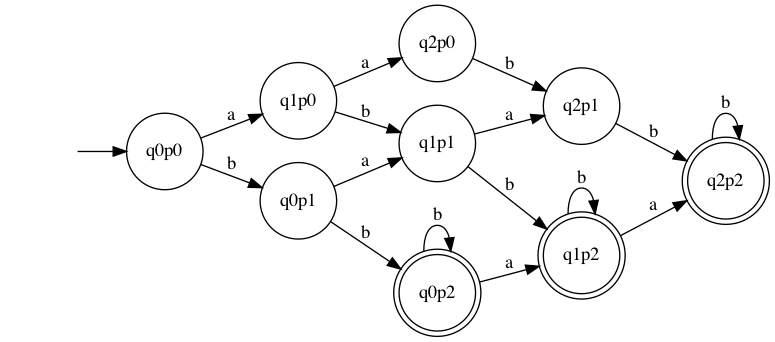
\includegraphics[width=0.8\textwidth]{g12.png}
\end{center}
 
%%%%%%%%%%%%%%% 1.3 %%%%%%%%%%%%%%%
\item {$L_3 = \{ w \in \{a,b\}^*  $ | $  |w|_a \neq |w|_b \} $} \\ \\
Конечный автомат нельзя построить, потому что требуется сравнивать количество символов $\Rightarrow$ нерегулярный язык.

%%%%%%%%%%%%%%% 1.4 %%%%%%%%%%%%%%%
\item {$L = \{ w \in \{a,b\}^*  $ | $ w w = w w w \}$} \\ \\
Язык из пустого символа.
\begin{center}
    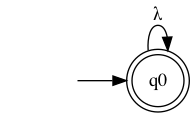
\includegraphics[width=0.3\textwidth]{g14.png}
\end{center}
\end{enumerate}





%%%%%%%%%%%%%%%%%%%%%%%%%%%%%% Задание 2 %%%%%%%%%%%%%%%%%%%%%%%%%%%%%%
\section{Задание №2. Построить конечный автомат, используя прямое произведение.}
\begin{enumerate}
%%%%%%%%%%%%%%% 2.1 %%%%%%%%%%%%%%%
\item {$L_1 = \{ w \in \{a,b\}^* $ | $ |w|_a \ge 2  \wedge   |w|_b \ge 2 \} \\ $} \\
$L_{11} = \{ w \in \{a,b\}^* $ | $ |w|_a \ge 2 \} \\$
\begin{center}
    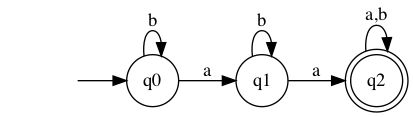
\includegraphics[width=0.5\textwidth]{g211.png}
\end{center}

$L_{12} = \{ w \in \{a,b\}^* $ | $ |w|_b \ge 2 \} \\$
\begin{center}
    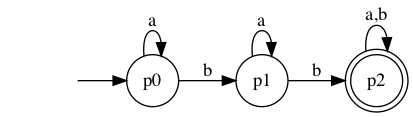
\includegraphics[width=0.5\textwidth]{g212.png}
\end{center}

\begin{center}
\[
    L_1 = L_{11} \times L_{12} \Rightarrow \]
    \[A_1 = \left\langle \sum_{1} , Q_1, S_1, T_1, \delta_1\right\rangle \quad 
    A_2 = \left\langle \sum_{2}, Q_2, S_2, T_2, \delta_2\right\rangle
\]

\[
    \sum = \{a, b\} \\
    Q = Q_1 \times Q_2 = \{q0p0, q0p1, q0p2, q1p0, q1p1, q1p2, q2p0, q2p1, q2p2\} \\
    S = \left\langle S_1, S_2 \right\rangle = \left\langle q0,p0 \right\rangle \\
    T = T_1 \times T_2 = \left\langle q2p2, q1p2, q0p2 \right\rangle
\]
\end{center}



\begin{center}
\begin{tabular}{ |c|c|c| } 
    \hline
    & $a$ & $b$ \\
    \hline
    \left\langle q0,p0 \right\rangle & \left\langle q1,p0 \right\rangle & \left\langle q0,p1 \right\rangle \\
    \hline
    \left\langle q0,p1 \right\rangle & \left\langle q1,p1 \right\rangle & \left\langle q0,p2 \right\rangle \\
    \hline
    \left\langle q0,p2 \right\rangle & \left\langle q1,p2 \right\rangle & \left\langle q0,p2 \right\rangle \\
    \hline
    \left\langle q1,p0 \right\rangle & \left\langle q2,p0 \right\rangle & \left\langle q1,p1 \right\rangle \\
    \hline
    \left\langle q1,p1 \right\rangle & \left\langle q2,p1 \right\rangle & \left\langle q1,p2 \right\rangle \\
    \hline
    \left\langle q1,p2 \right\rangle & \left\langle q2,p2 \right\rangle & \left\langle q1,p2 \right\rangle \\
    \hline
    \left\langle q2,p0 \right\rangle & \left\langle q2,p0 \right\rangle & \left\langle q2,p1 \right\rangle \\
    \hline
    \left\langle q2,p1 \right\rangle & \left\langle q2,p1 \right\rangle & \left\langle q2,p2 \right\rangle \\
    \hline
    (q2,p2) & (q2,p2) & (q2,p2) \\
    \hline
\end{tabular}
\end{center}

\begin{center}
    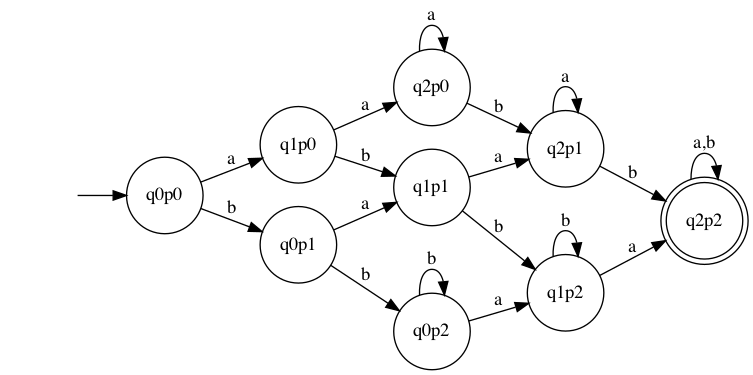
\includegraphics[width=0.8\textwidth]{g21.png}
\end{center}
%%%%%%%%%%%%%%% 2.2 %%%%%%%%%%%%%%%
\item {$L_2 = \{ w \in \{a,b\}^* $ | $ |w| \ge 3 \wedge |w| \text{ нечётное}\} $} \\ \\
$L_{21} = \{ w \in \{a,b\}^* $ | $ |w| \ge 3 \} \\$
\begin{center}
    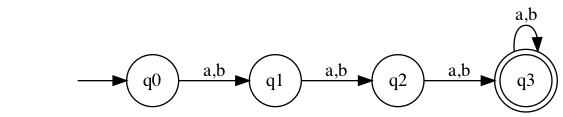
\includegraphics[width=0.8\textwidth]{g221.png}
\end{center}

$L_{22} = \{ w \in \{a,b\}^* $ | $ |w| \text{ нечётное}\} \\$
\begin{center}
    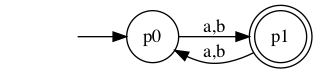
\includegraphics[width=0.5\textwidth]{g222.png}
\end{center}

\begin{center}
\[
    L_2 = L_{21} \times L_{22} \Rightarrow \]
    \[A_1 = \left\langle \sum_{1} , Q_1, S_1, T_1, \delta_1\right\rangle \quad 
    A_2 = \left\langle \sum_{2}, Q_2, S_2, T_2, \delta_2\right\rangle
\]

\[
    \sum = \{a, b\} \\
    Q = \{q0p0, q0p1, q1p0, q1p1, q2p0, q2p1, q3p0, q3p1\} \\
    S = \left\langle q0,p0 \right\rangle \\
    T = \left\langle q3,p1 \right\rangle \\
\]




\begin{tabular}{ |c|c|c| } 
    \hline
    & $a$ & $b$ \\
    \hline
    \left\langle q0,p0 \right\rangle & \left\langle q1,p1 \right\rangle & \left\langle q1,p1 \right\rangle \\
    \hline
    \left\langle q0,p1 \right\rangle & \left\langle q1,p0 \right\rangle & \left\langle q1,p0 \right\rangle \\
    \hline
    \left\langle q1,p0 \right\rangle & \left\langle q2,p1 \right\rangle & \left\langle q2,p1 \right\rangle \\
    \hline
    \left\langle q1,p1 \right\rangle & \left\langle q2,p0 \right\rangle & \left\langle q2,p0 \right\rangle \\
    \hline
    \left\langle q2,p0 \right\rangle & \left\langle q3,p1 \right\rangle & \left\langle q3,p1 \right\rangle \\
    \hline
    \left\langle q2,p1 \right\rangle & \left\langle q3,p0 \right\rangle & \left\langle q3,p0 \right\rangle \\
    \hline
    \left\langle q3,p0 \right\rangle &  \left\langle q3p,1 \right\rangle & \left\langle q3,p1 \right\rangle \\
    \hline
    \left\langle q3,p1 \right\rangle &  \left\langle q3,p0 \right\rangle & \left\langle q3,p0 \right\rangle \\
    \hline
\end{tabular}
\end{center}
\begin{center}
    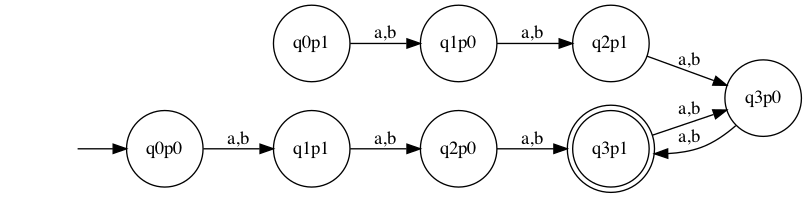
\includegraphics[width=0.8\textwidth]{g22.png}
\end{center}
Упрощаем:
\begin{center}
    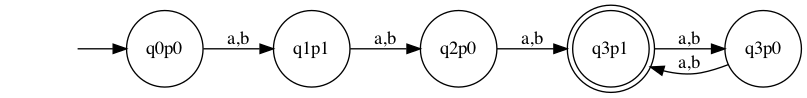
\includegraphics[width=0.8\textwidth]{g22_easy.png}
\end{center}

%%%%%%%%%%%%%%% 2.3 %%%%%%%%%%%%%%%
\item {$L_3 = \{w \in \{a,b\}^* $ | $ |w|_a \text{ чётно} \wedge |w|_b \text{ кратно трём} \} $} \\ \\
$L_{31} = \{w \in \{a,b\}^* $ | $ |w|_a \text{ чётно} \} $\\
\begin{center}
    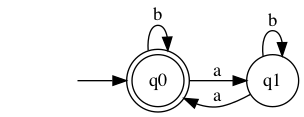
\includegraphics[width=0.5\textwidth]{g231.png}
\end{center}
$L_{32} = \{w \in \{a,b\}^* $ | $ |w|_b \text{ кратно трём} \} $\\
\begin{center}
    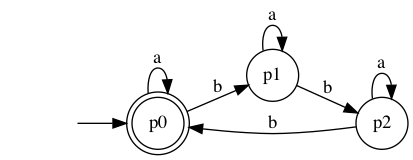
\includegraphics[width=0.5\textwidth]{g232.png}
\end{center}

\begin{center}
\[
    L_3 = L_{31} \times L_{32} \Rightarrow \]
    \[A_1 = \left\langle \sum_{1} , Q_1, S_1, T_1, \delta_1\right\rangle \quad 
    A_2 = \left\langle \sum_{2}, Q_2, S_2, T_2, \delta_2\right\rangle
\]

\[
    \sum = \{a, b\} \\
    Q = \{q0p0, q0p1, q0p2, q1p0, q1p1, q1p2\} \\
    S = \left\langle q0,p0 \right\rangle \\
    T = \left\langle q0,p0 \right\rangle \\
\]

\begin{tabular}{ |c|c|c| } 
    \hline
    & $a$ & $b$ \\
    \hline
    \left\langle q0,p0 \right\rangle & \left\langle q1,p0 \right\rangle & \left\langle q0,p1 \right\rangle \\
    \hline
    \left\langle q0,p1 \right\rangle & \left\langle q1,p1 \right\rangle & \left\langle q0,p2 \right\rangle \\
    \hline
    \left\langle q0,p2 \right\rangle & \left\langle q1,p2 \right\rangle & \left\langle q0,p0 \right\rangle \\
    \hline
    \left\langle q1,p0 \right\rangle & \left\langle q0,p0 \right\rangle & \left\langle q1,p1 \right\rangle \\
    \hline
    \left\langle q1,p1 \right\rangle & \left\langle q0,p1 \right\rangle & \left\langle q1,p2 \right\rangle \\
    \hline
    \left\langle q1,p2 \right\rangle & \left\langle q0,p2 \right\rangle & \left\langle q1,p0 \right\rangle \\
    \hline
\end{tabular}
\end{center}
\begin{center}
    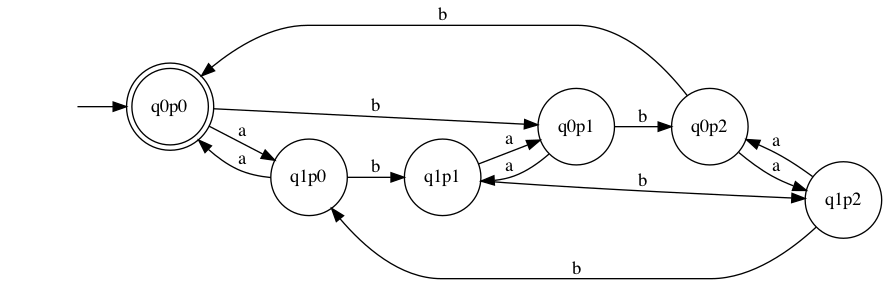
\includegraphics[width=0.8\textwidth]{g23.png}
\end{center}


%%%%%%%%%%%%%%% 2.4 %%%%%%%%%%%%%%%
\item {$L_4 = \overline{L_3}$\\} \\ \\
\text{Конечные вершины} \longleftrightarrow \text{начальные вершины}
\begin{center}
    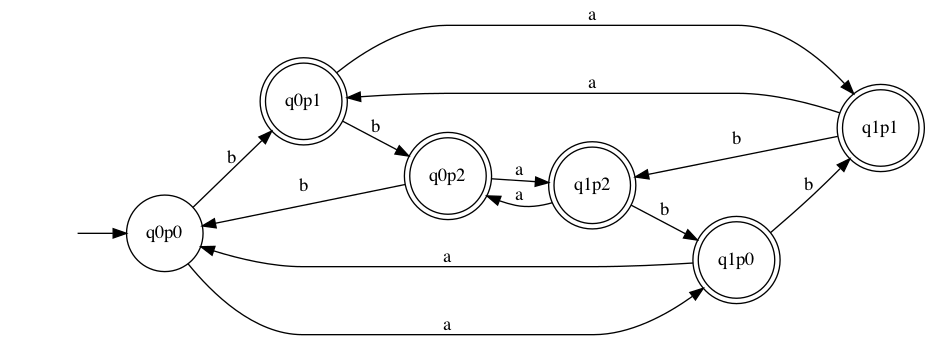
\includegraphics[width=0.8\textwidth]{g24.png}
\end{center}

%%%%%%%%%%%%%%% 2.5 %%%%%%%%%%%%%%%
5. $L_5 = L_2 \setminus L_3 = L_2 \wedge L_4 $ \\ \\
\begin{center}
    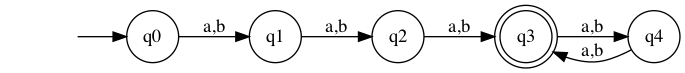
\includegraphics[width=0.5\textwidth]{g251.png}
    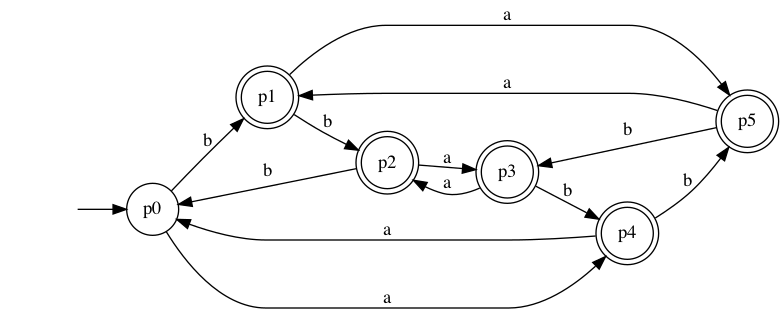
\includegraphics[width=0.5\textwidth]{g252.png}
\end{center}

\begin{center}
\[
    \sum = \{a, b\} \\
    S = \left\langle q0,p0 \right\rangle \\
    T = \{q3p1, q3p2, q3p3, q3p4, q3p5\}
\]
\end{center}
        \begin{center}
            \begin{tabular}{ |c|c|c| } 
            \hline
            & $a$ & $b$ \\
            \hline
            00 & 14 & 11\\
            \hline
            01 & 15 & 12\\
            \hline
            02 & 13 & 10\\
            \hline
            03 & 12 & 14\\
            \hline
            04 & 10 & 15\\
            \hline
            05 & 11 & 13\\
            \hline
            10 & 24 & 21\\
            \hline
            11 & 25 & 22\\
            \hline
            12 & 23 & 20\\
            \hline
            13 & 22 & 24\\
            \hline
            14 & 20 & 25\\
            \hline
            15 & 21 & 23\\
            \hline
            20 & 34 & 31\\
            \hline
            21 & 35 & 32\\
            \hline
            22 & 33 & 30\\
            \hline
            23 & 32 & 34\\
            \hline
            24 & 30 & 35\\
            \hline
            25 & 31 & 33\\
            \hline
            30 & 44 & 41\\
            \hline
            31 & 45 & 42\\
            \hline
            32 & 43 & 40\\
            \hline
            33 & 42 & 44\\
            \hline
            34 & 30 & 45\\
            \hline
            35 & 41 & 43\\
            \hline
            40 & 34 & 51\\
            \hline
            41 & 35 & 32\\
            \hline
            42 & 33 & 30\\
            \hline
            43 & 32 & 34\\
            \hline
            44 & 30 & 35\\
            \hline
            45 & 31 & 33\\
            \hline
            \end{tabular}
        \end{center} 
\begin{center}
    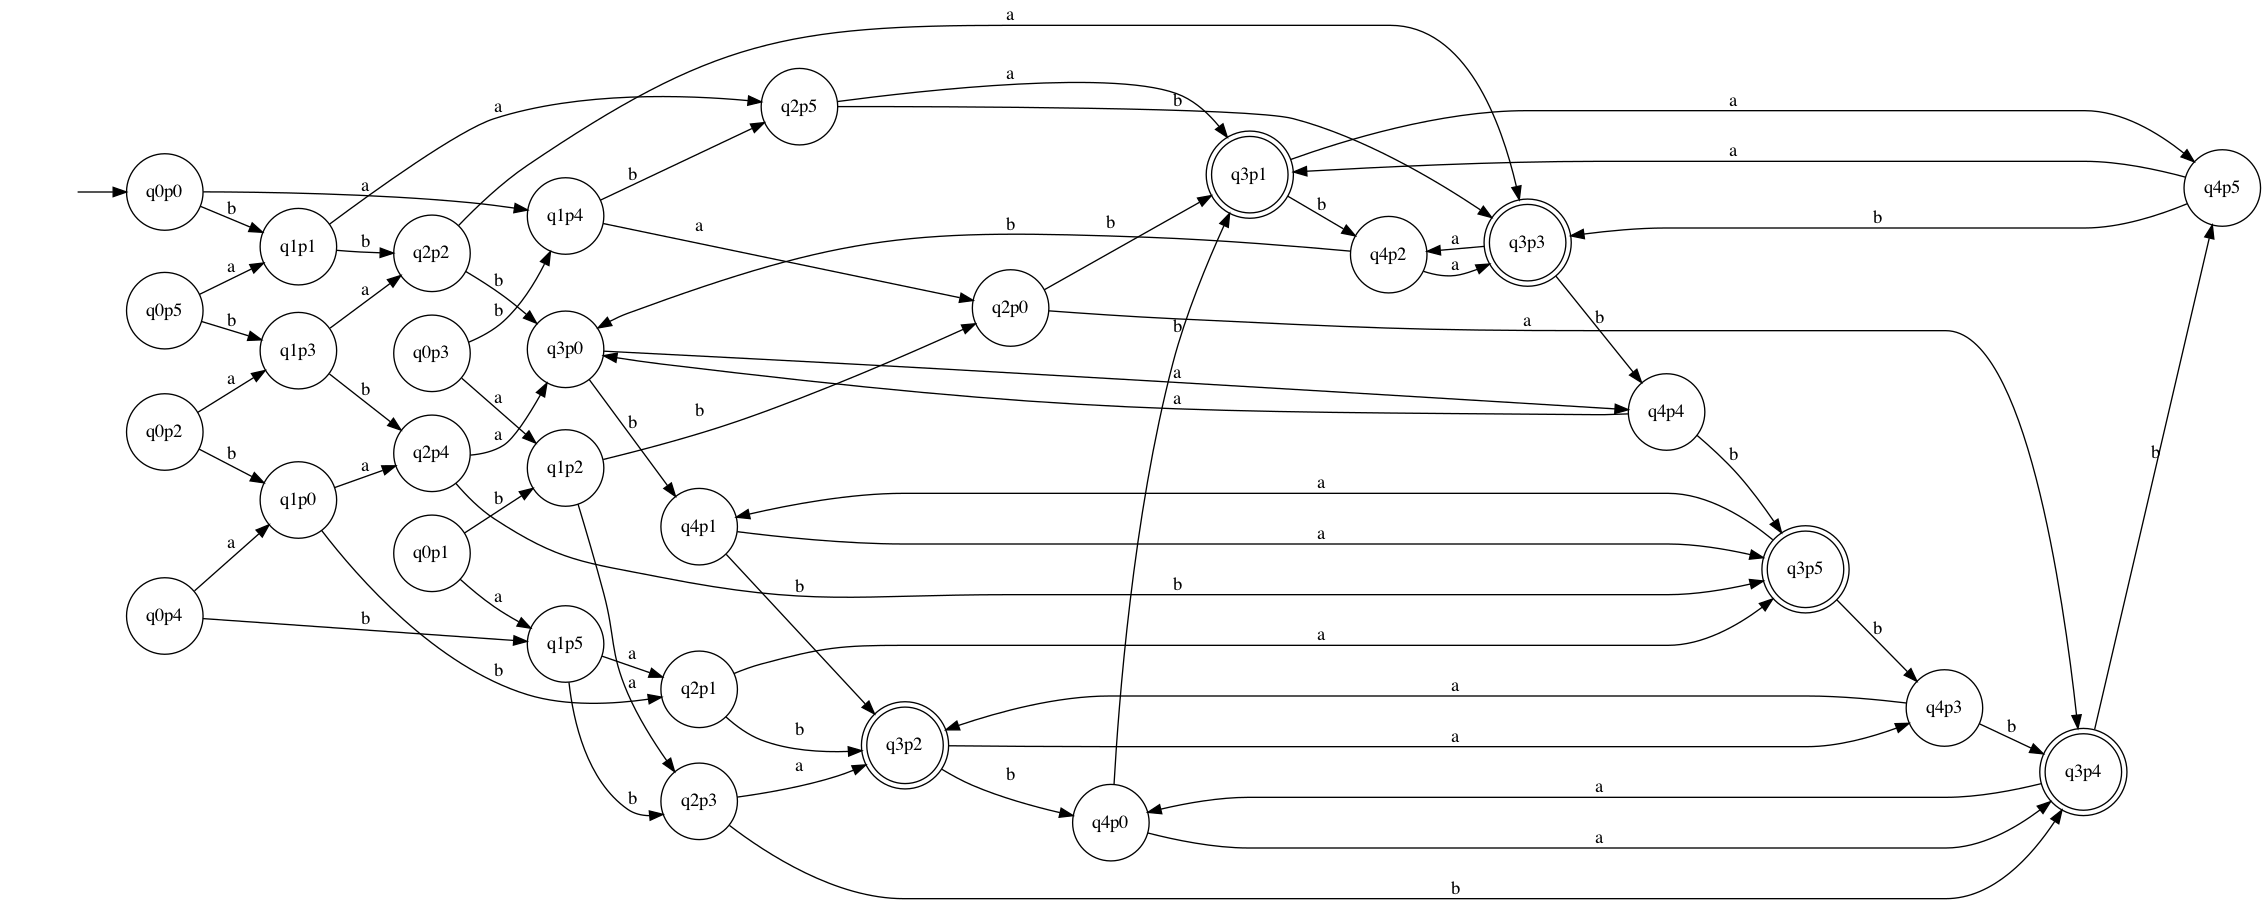
\includegraphics[width=1\textwidth]{g25.png}
\end{center}
\end{enumerate}









%%%%%%%%%%%%%%%%%%%%%%%%%%%%%% Задание 3 %%%%%%%%%%%%%%%%%%%%%%%%%%%%%%
\section{Задание №3. Построить минимальный ДКА по регулярному выражению.}

\begin{enumerate}

%%%%%%%%%%%%%%% 3.1 %%%%%%%%%%%%%%%
\item {$ (a b +a b a)^*a $} \\ \\
НКА с $\lambda$-переходами:
\begin{center}
    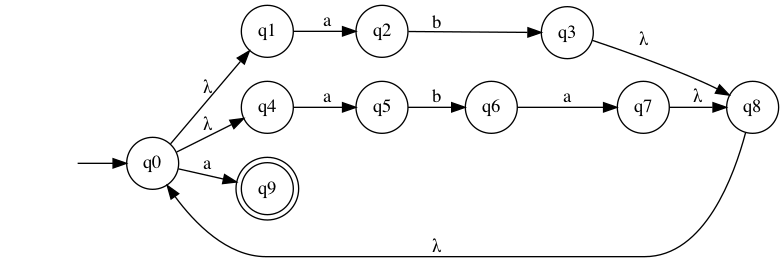
\includegraphics[width=0.8\textwidth]{g31_nka.png}
\end{center}

\begin{center}
    \begin{tabular}{|c|c|c|}
        \hline
        Q & a & b \\
        \hline
        q0 & q2 q5 q9 & - \\
        \hline
        q2 q5 q9 & - & q3 q6 \\
        \hline
        q3 q6 & q7 q2 q5 q9 & - \\
        \hline
        q7 q2 q5 q9 & q2 q5 q9 & q3 q6 \\
        \hline
    \end{tabular}\\
\end{center}
    
ДКА:
\begin{center}
    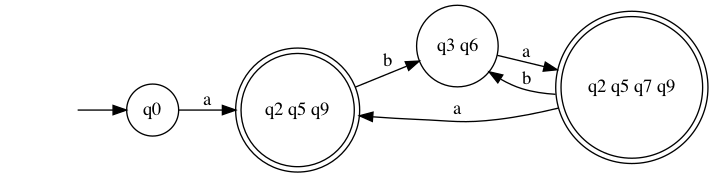
\includegraphics[width=0.8\textwidth]{g31.png} \\
\end{center}

%%%%%%%%%%%%%%% 3.2 %%%%%%%%%%%%%%%
\item {$ a(a(ab)^*b)^*(ab)^* $} \\ \\
НКА с $\lambda$-переходами:
\begin{center}
    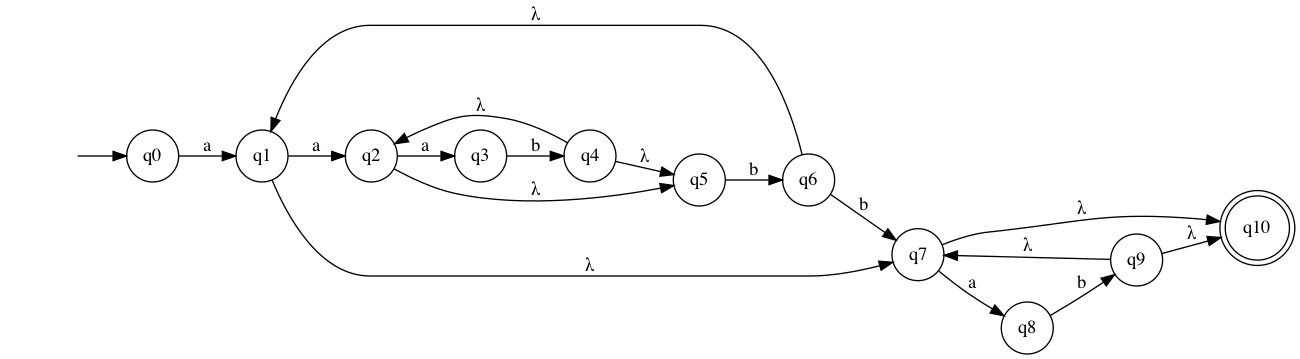
\includegraphics[width=0.8\textwidth]{g32_nka.png}
\end{center}

\end{enumerate}
\end{document}